\scanpage{57}
% archive foliation: 59
un pt de $K$ d'ordre $\geq2$, ou d'ordre 1 :

\uline{Lemme 2} Soit $K$ un segment topologique $\subset\mathbb C$,
et $x\in K$. \inserted{On suppose $K$ assez régulier (rectifiable suffit ??)} Alors

a) Si $x$ n'est pas extrémité de $K$, alors il existe
\deleted{un voisinage \inserted{ouvert} $U$ de $x$ dans $\mathbb C$, ne contenant pas
d'extrémités de $\unsure{U|K}$, tel que $U\setminus K\cap U$
ait deux composantes connexes $U'$ et $U''$
avec $\overline{U'}\cap U=U'\cup(K\cap U)$, $\overline{U''}\cap U=U''\cup(K\cap U)$, et
\unsure{fonction holo}}

\figure{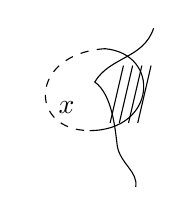
\begin{tikzpicture}[scale=.65]
\draw[dashed] (-.1,1.1) .. controls (-1.6,1) and (-1.6,-.5) .. (-.4,-.5);
\draw (-.4,-.5) .. controls (.9,-.5) and (1,1) .. (-.1,1.1);
\draw (.85,1.5) .. controls (.65,.9) and (.0,.95) .. (-.3,.45)
.. controls (.05,.2) and (.1,-.5) .. (.14,-.8)
.. controls (.2,-1.15) and (.55,-1.3) .. (.5,-1.6);
\foreach \x in {0,.18,.36,.54} {\draw (\x,-.35)--({\x+.26},.77);}
\node at (-.85,-.05) {$x$};
\end{tikzpicture}}

\deleted{\unsure{$f$}} une application continue injective
\inserted{de $\deleted{\unsure{\mathbb C}}H\cap\mathbb D^\circ\longrightarrow\mathbb C$},
\deleted{de $H\cap\mathbb D^\circ$ dans $\mathbb C$, hol. dans $H\cap$
$\mathbb D^\circ\subset\mathbb C$, continue}
holomorphe dans \deleted{$\unsure{\mathbb D\setminus H\supset\mathbb R}$}
\inserted{$(\operatorname{Int}H)\cap\mathbb D^\circ$},
\deleted{$=\,]-1,+1[\quad(\unsure{\ne}\ \mathbb D^{++}\amalg \mathbb D^{--})$}
\deleted{(mais pas \unsure{néct}\ dans deux plans $\mathbb R$)}
(mais pas néc \unsure{hol. au vts de}\ \deleted{dans}
$\delta H\cap\mathbb D^\circ=\,]-1,+1[)$ telle que
$f(\delta H\cap\mathbb D^\circ)\subset K$ et
$f(0)=x$. De plus, pour une rive donnée de
$K$ en $x$, OPS que cette rive est celle déterminée
par \inserted{$\operatorname{Im}f=$} $f(H\cap\mathbb D^\circ)$.

b) Si $x$ est extrémité de $K$, alors $\exists$
$f:H\cap\mathbb D^\circ\longrightarrow\mathbb C$, hol. \inserted{\deleted{et topologique}}
dans $(\operatorname{Int}H)\cap\mathbb D^\circ$, \deleted{et}
\deleted{injective dans $\unsure{\mathbb D^\circ}$ telle que
$\unsure{\{f(-t)=f(t)}$ $\unsure{\{\}}$}
\deleted{\unsure{soit en}\ $f$}
\inserted{telle que $f(0)=0$}
\deleted{$\unsure{f\,]-1,0)}$}
\deleted{$f\mid[-1,0]$ et $f\mid[0,1[$ soient injectifs,}

\figure{\begin{tikzpicture}[scale=.65]
\draw (-.08,2.4).. controls (-.6,1.7) and (.15,1.2) ..(-.25,.65)
..controls(-.7,.2)and(-.08,-.1)..(-.22,-.75);
\draw[dashed](-.85,-.7) arc[start angle=145,end angle=35,radius=1];
\draw (-1.05,-1.35) .. controls (-1.25,-2.25) and (.15,-2.8) .. (.7,-1.95);
\draw (.7,-1.95)..controls(1.1,-1.3)and(.9,-.85)..(.65,-.75);
\node at (-.25,-1.35) {$x$};
\end{tikzpicture}}
